\chapter{Analysis}
\label{chap:analysis}

In diesem Abschnitt wird eine grobe Übersicht über die Software erstellt. Fragen wie, was sind die Anforderungen an die Software, was sind die Anforderungen der Akteure etc. werden hier beantwortet. Ebenfalls wird eine grobe Übersicht über die Programmstruktur erstellt.

\section{Domainmodel}
\label{sec:domain_model}
In diesem Abschnitt wird das Domain Model ("{}Fachmodell"{}) des Mindmap Programmes beschrieben. Es stellt die 
wichtigsten Fachklassen und Assoziationen dar und zeigt die jeweiligen Multiplizitäten.

\begin{figure}[H]
	\centering
		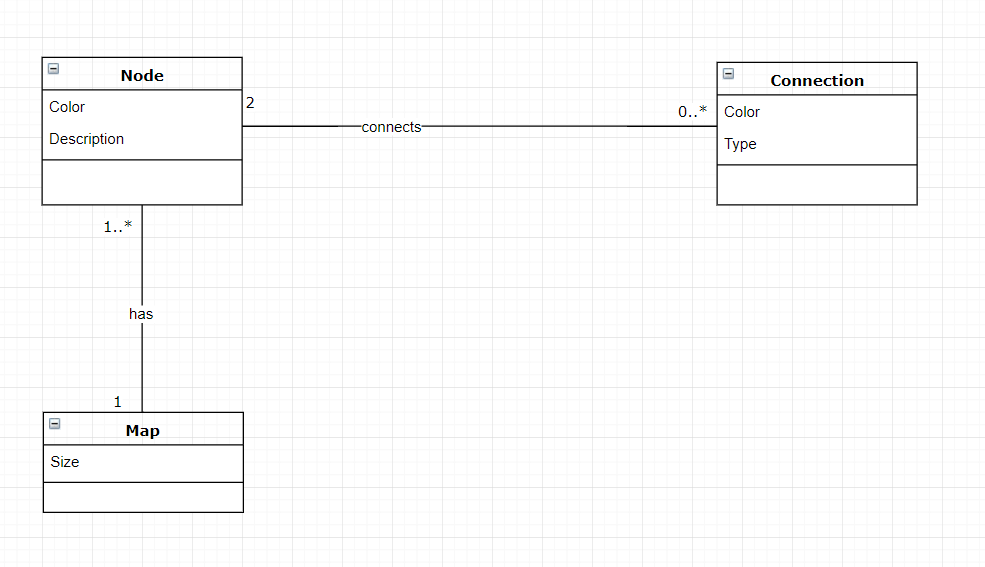
\includegraphics[scale=0.7]{images/DomainModel.png}
	\caption{Domainmodel}
	\label{fig:domain_model}
\end{figure}

Wie oben in der Grafik zu sehen ist, haben wir uns dafür entschieden, dass eine Map mindestens einen Knoten haben muss um eine Map zu sein. Im Moment denken wir das die Connection und die Map keine direkte Verbindung benötigen dies könnte sich aber beim Implementieren vielleicht noch ändern. Ebenfalls haben wird definiert, dass eine Verbindung immer zwischen 2 Knoten besteht.

\subsection{Assoziationen}
\label{subsec:assoziationen}
\begin{itemize}
\item Zwei Knoten haben keine oder mehrere Verbindungen. Eine Verbindung besteht aus 2 Knoten.
\item Eine Map hat einen oder Mehrere Knoten. Ein Knoten gehört zu einer Map.
\end{itemize}

\section{Use Cases}
\label{sec:use_cases}
Use-Cases beschreiben die Requirements der einzelnen Akteure, es zeigt die Abläufe des Programmes auf. Zeigt dabei aber nicht wie die einzelnen Teile funktionieren.

Eine Liste der Use Cases befindet sich im Anhang \ref{chap:use_cases}.

\subsection{Use Case Diagramm}
\label{subsec:use_case_diagramm}

\begin{figure}[H]
	\centering
		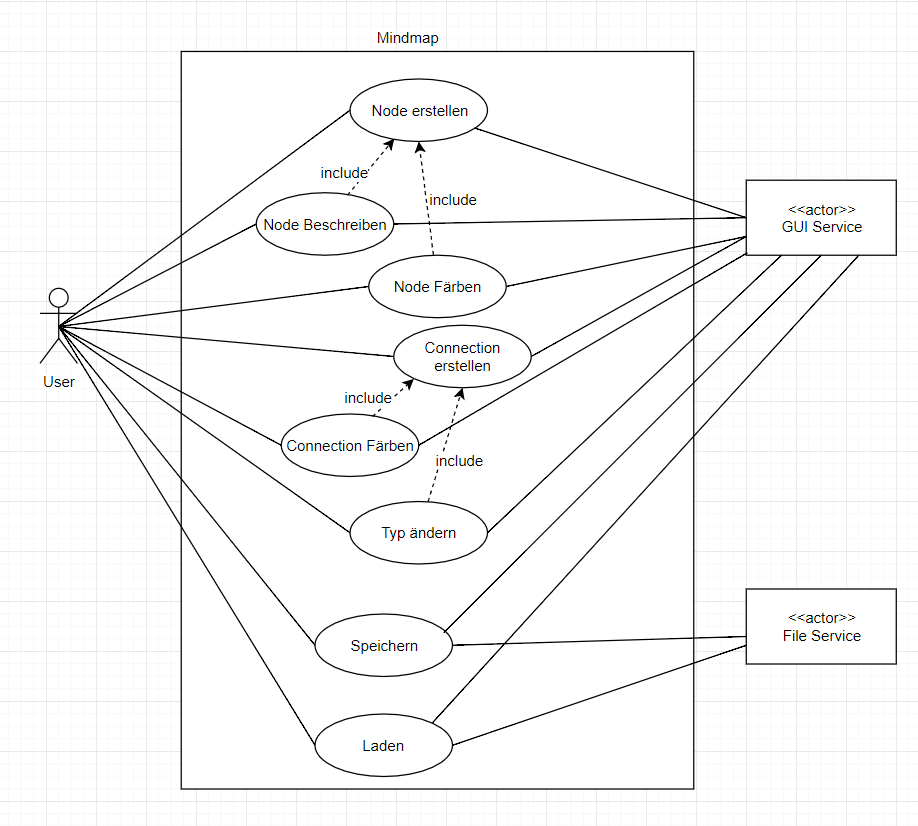
\includegraphics[scale=0.7]{images/UseCaseDiagram.PNG}
	\caption{Use Case Diagramm}
	\label{fig:use_case_diagramm}
\end{figure}

\subsection{Mindmap Process}
\label{subsec:mindmap_process}
Neues Mindmap Szenario:
\begin{enumerate}
\item Benutzer erstellt neues Mindmap
\item GUI Service zeigt leeres Mindmap an
\item Benutzer erstellt Nodes und Connections 
\item Benutzer bearbeitet die Nodes und Connections z.B. Typ, Beschreibung, Farbe.
\item GUI Service stellt dies dar
\item Punkt 3-5 werden wiederholt bis der Benutzer zufrieden ist
\item Benutzer speichert seine Arbeit
\item GUI Service übergibt Fileservice die Map
\item Fileservice speichert die Map in ein Dokument
\end{enumerate}

Mindmap bearbeiten Szenario: 
\begin{enumerate}
\item Benutzer lädt Mindmap
\item Fileservice lädt das alte Mindmap
\item GUI Service zeigt das Mindmap an (Danach analog zu oberem Szenario)
\end{enumerate}

\section{User Stories}
\label{sec:user_stories}
Eine User-Story beschreibt in ein oder zwei Sätzen eine gewünschte Funktion des Programmes.
\begin{enumerate}
\item Als Benutzer möchte ich, dass das Programm selbsterklärend und einfach zu bedienen ist.
\item Als Benutzer möchte ich ein Programm welches schnell startet und sich nicht langsam anfühlt.
\item Als Benutzer möchte ich ein optisch Ansprechendes Design. Als Benutzer finde ich ein Programm
besser wenn sein Design State of the Art ist.
\item Als Benutzer möchte ich, dass das Mindmap auf dem Papier gleich aussieht wie es im Programm ausgesehen hat.
\item Als Benutzer möchte ich nicht einen Experten konsultieren müssen um ein so triviales Programm zu installieren. 
\item Als Benutzer möchte ich mit dem Programm neue Mindmaps erstellen können.
\item Als Benutzer möchte ich neue Knoten hinzufügen können, welcher eine Beschreibung besitzt und wenn gewünscht auch eine spezielle Farbe haben kann. 
\item Als Benutzer möchte ich die verschiedenen Informationen, also Knoten miteinander vernetzen und so gruppieren können. 
\item Als Benutzer möchte ich meine Arbeit speichern können und gespeicherte Projekte auch wieder laden können
\item Als Benutzer möchte ich die Beschreibung eines Knoten auch nach seiner Erstellung bearbeiten können.
\item Als Benutzer möchte ich die Farbe eines Knotens nach seiner Erstellung bearbeiten können.
\item Als Benutzer möchte ich verschiedene Verbindungstypen definieren können, ich möchte Verbindungen zwischen verschiedenen Themen speziell hervorheben können. 
\item Als Benutzer möchte ich mein Mindmap drucken können.
\item Als Benutzer möchte ich mein Mindmap exportieren können, um es zum Beispiel als Bilddatei in einem Worddokument einfügen zu können.
\item Als Benutzer möchte ich ein Mindmap mit möglichst wenigen überschneidenden Verbindungen, das Programm sollte eine Möglichkeit bieten dieses Problem zu lösen.
\end{enumerate}

\section{Systemkontext}
\label{sec:systemkontext}
Der Systemkontext ist eine Beschreibung des Systems, seiner Teile und äusserlichen Einwirkungen auf das System.

Der Benutzer kann mit unserer Software ein Mindmap erstellen. Dies geschieht über eine grafische Benutzeroberfläche. Mit Hilfe eines Algorithmus können die Themen und Verbindungen des Mindmap optimal verteilt werden. Die Benutzeroberfläche und der Algorithmus sind Teil der Software\\
Die Software greift auf das Dateisystem des Computers zu um ein Mindmap zu speichern oder zu laden. Der Druckservice des Computers erlaubt das Drucken des Mindmaps. Diese beiden Teile liegen ausserhalb unserer Software.

\begin{figure}[H]
	\centering
		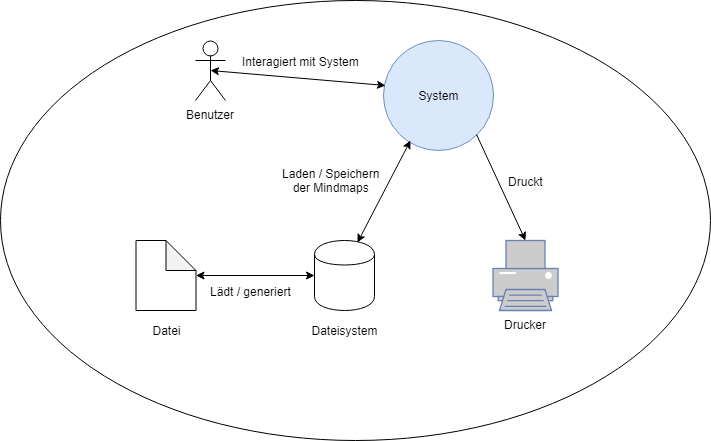
\includegraphics[scale=0.7]{images/Systemkontext.png}
	\caption{Systemkontext}
	\label{fig:systemkontext}
\end{figure}

\section{Anforderungen}
\label{sec:anforderungen}
--> Teil Modul Requirements Engineering
